\documentclass{ximera}
\usepackage{longdivision}
\usepackage{polynom}
\usepackage{float}% Use `H' as the figure optional argument to force it's vertical placement to conform to source.
%\usepackage{caption}% Allows us to describe the figures without having "figure 1:" in it. :: Apparently Caption isn't supported.
%    \captionsetup{labelformat=empty}% Actually does the figure configuration stated above.
\usetikzlibrary{arrows.meta,arrows}% Allow nicer arrow heads for tikz.
\usepackage{gensymb, pgfplots}
\usepackage{tabularx}
\usepackage{arydshln}
\usepackage[margin=1.5cm]{geometry}
\usepackage{indentfirst}

\setlength\parindent{16pt}

\graphicspath{
  {./}
  {./explorePolynomials/}
  {./exploreRadicals/}
  {./graphing/}
}

%% Default style for tikZ
\pgfplotsset{my style/.append style={axis x line=middle, axis y line=
middle, xlabel={$x$}, ylabel={$y$}, axis equal }}


%% Because log being natural log is too hard for people.
\let\logOld\log% Keep the old \log definition, just in case we need it.
\renewcommand{\log}{\ln}


%%% Changes in polynom to show the zero coefficient terms
\makeatletter
\def\pld@CF@loop#1+{%
    \ifx\relax#1\else
        \begingroup
          \pld@AccuSetX11%
          \def\pld@frac{{}{}}\let\pld@symbols\@empty\let\pld@vars\@empty
          \pld@false
          #1%
          \let\pld@temp\@empty
          \pld@AccuIfOne{}{\pld@AccuGet\pld@temp
                            \edef\pld@temp{\noexpand\pld@R\pld@temp}}%
           \pld@if \pld@Extend\pld@temp{\expandafter\pld@F\pld@frac}\fi
           \expandafter\pld@CF@loop@\pld@symbols\relax\@empty
           \expandafter\pld@CF@loop@\pld@vars\relax\@empty
           \ifx\@empty\pld@temp
               \def\pld@temp{\pld@R11}%
           \fi
          \global\let\@gtempa\pld@temp
        \endgroup
        \ifx\@empty\@gtempa\else
            \pld@ExtendPoly\pld@tempoly\@gtempa
        \fi
        \expandafter\pld@CF@loop
    \fi}
\def\pld@CMAddToTempoly{%
    \pld@AccuGet\pld@temp\edef\pld@temp{\noexpand\pld@R\pld@temp}%
    \pld@CondenseMonomials\pld@false\pld@symbols
    \ifx\pld@symbols\@empty \else
        \pld@ExtendPoly\pld@temp\pld@symbols
    \fi
    \ifx\pld@temp\@empty \else
        \pld@if
            \expandafter\pld@IfSum\expandafter{\pld@temp}%
                {\expandafter\def\expandafter\pld@temp\expandafter
                    {\expandafter\pld@F\expandafter{\pld@temp}{}}}%
                {}%
        \fi
        \pld@ExtendPoly\pld@tempoly\pld@temp
        \pld@Extend\pld@tempoly{\pld@monom}%
    \fi}
\makeatother




%%%%% Code for making prime factor trees for numbers, taken from user Qrrbrbirlbel at: https://tex.stackexchange.com/questions/131689/how-to-automatically-draw-tree-diagram-of-prime-factorization-with-latex

\usepackage{forest,mathtools,siunitx}
\makeatletter
\def\ifNum#1{\ifnum#1\relax
  \expandafter\pgfutil@firstoftwo\else
  \expandafter\pgfutil@secondoftwo\fi}
\forestset{
  num content/.style={
    delay={
      content/.expanded={\noexpand\num{\forestoption{content}}}}},
  pt@prime/.style={draw, circle},
  pt@start/.style={},
  pt@normal/.style={},
  start primeTree/.style={%
    /utils/exec=%
      % \pt@start holds the current minimum factor, we'll start with 2
      \def\pt@start{2}%
      % \pt@result will hold the to-be-typeset factorization, we'll start with
      % \pgfutil@gobble since we don't want a initial \times
      \let\pt@result\pgfutil@gobble
      % \pt@start@cnt holds the number of ^factors for the current factor
      \def\pt@start@cnt{0}%
      % \pt@lStart will later hold "l"ast factor used
      \let\pt@lStart\pgfutil@empty,
    alias=pt-start,
    pt@start/.try,
    delay={content/.expanded={$\noexpand\num{\forestove{content}}
                            \noexpand\mathrlap{{}= \noexpand\pt@result}$}},
    primeTree},
  primeTree/.code=%
    % take the content of the node and save it in the count
    \c@pgf@counta\forestove{content}\relax
    % if it's 2 we're already finished with the factorization
    \ifNum{\c@pgf@counta=2}{%
      % add the factor
      \pt@addfactor{2}%
      % finalize the factorization of the result
      \pt@addfactor{}%
      % and set the style to the prime style
      \forestset{pt@prime/.try}%
    }{%
      % this simply calculates content/2 and saves it in \pt@end
      % this is later used for an early break of the recursion since no factor
      % can be greater then content/2 (for integers of course)
      \edef\pt@content{\the\c@pgf@counta}%
      \divide\c@pgf@counta2\relax
      \advance\c@pgf@counta1\relax % to be on the safe side
      \edef\pt@end{\the\c@pgf@counta}%
      \pt@do}}

%%% our main "function"
\def\pt@do{%
  % let's test if the current factor is already greather then the max factor
  \ifNum{\pt@end<\pt@start}{%
    % great, we're finished, the same as above
    \expandafter\pt@addfactor\expandafter{\pt@content}%
    \pt@addfactor{}%
    \def\pt@next{\forestset{pt@prime/.try}}%
  }{%
    % this calculates int(content/factor)*factor
    % if factor is a factor of content (without remainder), the result will
    % equal content. The int(content/factor) is saved in \pgf@temp.
    \c@pgf@counta\pt@content\relax
    \divide\c@pgf@counta\pt@start\relax
    \edef\pgf@temp{\the\c@pgf@counta}%
    \multiply\c@pgf@counta\pt@start\relax
    \ifNum{\the\c@pgf@counta=\pt@content}{%
      % yeah, we found a factor, add it to the result and ...
      \expandafter\pt@addfactor\expandafter{\pt@start}%
      % ... add the factor as the first child with style pt@prime
      % and the result of int(content/factor) as another child.
      \edef\pt@next{\noexpand\forestset{%
        append={[\pt@start, pt@prime/.try]},
        append={[\pgf@temp, pt@normal/.try]},
        % forest is complex, this makes sure that for the second child, the
        % primeTree style is not executed too early (there must be a better way).
        delay={
          for descendants={
            delay={if n'=1{primeTree, num content}{}}}}}}%
    }{%
      % Alright this is not a factor, let's get the next factor
      \ifNum{\pt@start=2}{%
        % if the previous factor was 2, the next one will be 3
        \def\pt@start{3}%
      }{%
        % hmm, the previos factor was not 2,
        % let's add 2, maybe we'll hit the next prime number
        % and maybe a factor
        \c@pgf@counta\pt@start
        \advance\c@pgf@counta2\relax
        \edef\pt@start{\the\c@pgf@counta}%
      }%
      % let's do that again
      \let\pt@next\pt@do
    }%
  }%
  \pt@next
}

%%% this builds the \pt@result macro with the factors
\def\pt@addfactor#1{%
  \def\pgf@tempa{#1}%
  % is it the same factor as the previous one
  \ifx\pgf@tempa\pt@lStart
    % add 1 to the counter
    \c@pgf@counta\pt@start@cnt\relax
    \advance\c@pgf@counta1\relax
    \edef\pt@start@cnt{\the\c@pgf@counta}%
  \else
    % a new factor! Add the previous one to the product of factors
    \ifx\pt@lStart\pgfutil@empty\else
      % as long as there actually is one, the \ifnum makes sure we do not add ^1
      \edef\pgf@tempa{\noexpand\num{\pt@lStart}\ifnum\pt@start@cnt>1 
                                           ^{\noexpand\num{\pt@start@cnt}}\fi}%
      \expandafter\pt@addfactor@\expandafter{\pgf@tempa}%
    \fi
    % setup the macros for the next round
    \def\pt@lStart{#1}% <- current (new) factor
    \def\pt@start@cnt{1}% <- first time
  \fi
}
%%% This simply appends "\times #1" to \pt@result, with etoolbox this would be
%%% \appto\pt@result{\times#1}
\def\pt@addfactor@#1{%
  \expandafter\def\expandafter\pt@result\expandafter{\pt@result \times #1}}

%%% Our main macro:
%%% #1 = possible optional argument for forest (can be tikz too)
%%% #2 = the number to factorize
\newcommand*{\PrimeTree}[2][]{%
  \begin{forest}%
    % as the result is set via \mathrlap it doesn't update the bounding box
    % let's fix this:
    tikz={execute at end scope={\pgfmathparse{width("${}=\pt@result$")}%
                         \path ([xshift=\pgfmathresult pt]pt-start.east);}},
    % other optional arguments
    #1
    % And go!
    [#2, start primeTree]
  \end{forest}}
\makeatother


\providecommand\tabitem{\makebox[1em][r]{\textbullet~}}
\providecommand{\letterPlus}{\makebox[0pt][l]{$+$}}
\providecommand{\letterMinus}{\makebox[0pt][l]{$-$}}

\renewcommand{\texttt}[1]{#1}% Renew the command to prevent it from showing up in the sage strings for some weird reason.
%\renewcommand{\text}[1]{#1}% Renew the command to prevent it from showing up in the sage strings for some weird reason.



\title{Practice Exam Problems (Sections 4-7)}
\begin{document}
\begin{abstract}
    This is the (non randomized) review to help check that the you have good footing on sections 4-7 before moving on. This is not intended to represent the length or plausible difficulty of an exam on this topic; it should help direct you to the sections where you are weakest/strongest in your studying.
\end{abstract}

\maketitle

\begin{javascript}
// Check to see if input is positive.
  function isPositive(number) {
    return number > 0;
  };




// Check to see if two inputs are the same parity in terms of even/odd.
  function sameParity(a,b) {
    return (a-b)%2 == 0;
  };




// Check to see if two strings match in a case-insensitive way.
  caseInsensitive = function(a,b) {
    return a.toLowerCase() == b.toLowerCase();
  };
  



// sameDerivative checks to see if the derivative with respect to x and c are equal.
  sameDerivative = function(a,b) {
    return (a.derivative('x').equals( b.derivative('x') ) && a.derivative('C').equals( b.derivative('C') )) ;
  };




// No idea what this is doing... demonstrating the ``promise'' feature maybe?
slowOdd = function(a) {
    return new Promise( function(resolve, reject) {
        if (a == 0)
            reject('I do not like zero.');
        else
            setTimeout(function(){
            resolve(a % 2 == 1);
            }, 1000);      
        });
    };


// Check to make sure each submitted answer is linear, and that the product of the answers is the expected function.
linearFactoring = function(correctAns) {
    var i;
    var Truth;
    var Prod;
    Truth=1;
    Prod=1;
        for (i = 1; i < arguments.length; i++) {
            Truth = Truth * arguments[i].derivative('x').derivative('x').equals(0)
            Prod = Prod * arguments[i]
        };
        Truth = Truth*(Prod.equals(correctAns))
        return Truth
    };




\end{javascript}


\begin{problem}
    In a residential neighborhood most families have multiple cars; at least one for each parent and maybe one for the kids over 16. You have learned to recognize every car in your neighborhood and which house it belongs to. What is the domain of this association (recognizing the car and then recalling which house it belongs to)?
    \begin{multipleChoice}
        \choice{The houses in the neighborhood.}
        \choice{Your individual neighbors.}
        \choice[correct]{The cars in the neighborhood.}
    \end{multipleChoice}
    \begin{problem}
        What is the codomain?
        \begin{multipleChoice}
            \choice[correct]{The houses in the neighborhood.}
            \choice{Your individual neighbors.}
            \choice{The cars in the neighborhood.}
        \end{multipleChoice}
        \begin{problem}
            Is this association a function?
            \begin{multipleChoice}
                \choice{No, each house has multiple cars.}
                \choice{No, each car belongs to multiple people.}
                \choice[correct]{Yes, each car belongs to one house.}
                \choice{Yes, each house has one car.}
            \end{multipleChoice}
        \end{problem}
    \end{problem}
\end{problem}

\begin{problem}
    You decide to plant pines trees to provide a privacy screen around a piece of your property. Use the following information to answer the questions.
    \begin{itemize}
        \item You choose white pine as it is a fast-growing variety.
        \item At the time of planting, the trees are all 2 feet tall.
        \item This species of tree grows an average of 2.7 feet per year.
        \item The land you wish to screen is 14 feet by 20 feet.
        \item You think pine trees are quite pretty.
    \end{itemize}
%%% Next two questions removed as they are for modeling, not the properties/functions section.
%    Which of these are pieces of data?
%    \begin{selectAll}
%        \choice {You choose white pine as it is a fast-growing variety.}
%        \choice[correct] {At the time of planting, the trees are 2 feet tall.}
%        \choice[correct] {The land you wish to screen is 14 feet by 20 feet.}
%        \choice {You think pine trees are quite pretty.}
%    \end{selectAll}
%
%    \begin{problem}
%        You would like to know how long it will take the trees to reach a sufficient height to screen your property from the road. Which pieces of information are relevant?
%        \begin{selectAll}
%            \choice [correct]{You choose white pine as it is a fast-growing variety; they grow an average of 2.7 feet per year.}
%            \choice[correct] {At the time of planting, the trees are 2 feet tall.}
%            \choice{The land you wish to screen is 14 feet by 20 feet.}
%            \choice {You think pine trees are quite pretty.}
%        \end{selectAll}

    \begin{problem}
        After looking up information you determine it is easiest to first figure out how high the trees will be (on average) each year, and then use that to determine how long you must wait. When writing a mathematical expression for this, what should the independent variable be?
        \begin{multipleChoice}
            \choice{The height of the trees.}
            \choice[correct]{The time in years.}
            \choice{The height of the trees at planting.}
        \end{multipleChoice}
        \begin{problem}
            Does this expression represent a function?
            \begin{multipleChoice}
                \choice{Yes, there are multiple trees to track per year.}
                \choice[correct]{Yes, for each year there is only one height that we are calculating (the average).}
                \choice{No, for each year this is only one height that we are calculating (the average).}
                \choice{No, multiple trees means there will be many different heights at the end of each year.}
                \choice{No, there are multiple years where trees could be the same height.}
            \end{multipleChoice}
            \begin{problem}
                Write an equation describing this relationship using $t$ for the time in years and $h$ for the height of the trees in feet. $\answer{h}$ = $\answer{2.7t+2}$
        
                \begin{problem}
                    Identify the domain, codomain, and whether this equation is a function.
                    \begin{multipleChoice}
                        \choice{\textbf{Domain: }height in feet; \\ \textbf{Codomain: }time in years; \\ \textbf{Is it a function? }yes}
                        \choice{\textbf{Domain: }time in years; \\ \textbf{Codomain: }height in feet; \\ \textbf{Is it a function? }no}
                        \choice{\textbf{Domain: }height in feet; \\ \textbf{Codomain: }time in years; \\ \textbf{Is it a function? }no}
                        \choice[correct]{\textbf{Domain: }time in years; \\ \textbf{Codomain: }height in feet; \\ \textbf{Is it a function? }yes}
                    \end{multipleChoice}
                \end{problem}
            \end{problem}
        \end{problem}
    \end{problem}
\end{problem}

\begin{problem}
    Does the following graph depict a function?
\begin{center}
    \begin{tikzpicture}
        \begin{axis}[my style, minor tick num=1]
            \addplot[domain=-3:5]{-abs(x-1)+3};
        \end{axis}
    \end{tikzpicture}
\end{center}

    \begin{multipleChoice}
        \choice[correct]{Function}
        \choice{Not a function}
    \end{multipleChoice}
\end{problem}


Use the following graph for Problems 4-7.
\begin{center}
    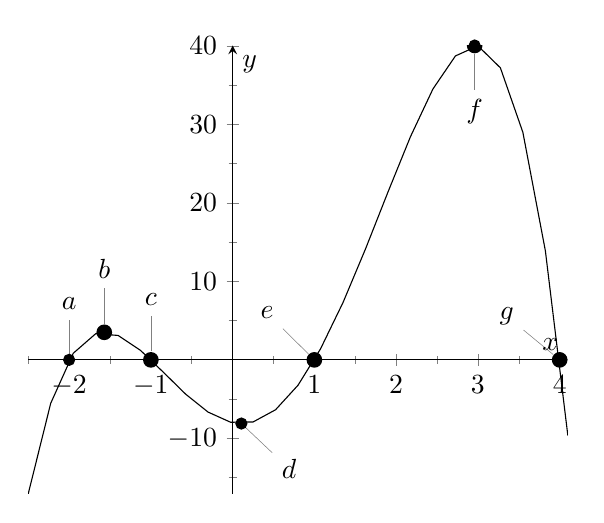
\begin{tikzpicture}[baseline={([yshift={-1ex}]current bounding box.north)}]
        \begin{axis}[axis x line=middle, axis y line=
        middle, xlabel={$x$}, ylabel={$y$}, minor tick num=1]
            \addplot[domain=-2.5:4.1]{-(x+1)*(x-1)*(x+2)*(x-4)};
            \addplot [mark=*, only marks] coordinates{(-1,0)(1,0)(-2,0)(4,0)(-1.57,3.51)(0.107,-8.11)(2.96,40.04)};
            \node[pin={90:{$a$}},circle,fill,inner sep=1pt] at (axis cs:-2,0) {};
            \node[pin={90:{$b$}},circle,fill,inner sep=2pt] at (axis cs:-1.57,3.51) {};
            \node[pin={90:{$c$}},circle,fill,inner sep=2pt] at (axis cs:-1,0) {};
            \node[pin={320:{$d$}},circle,fill,inner sep=1pt] at (axis cs:0.107,-8.11) {};
            \node[pin={135:{$e$}},circle,fill,inner sep=2pt] at (axis cs:1,0) {};
            \node[pin={270:{$f$}},circle,fill,inner sep=2pt] at (axis cs:2.96,40.04) {};
            \node[pin={145:{$g$}},circle,fill,inner sep=2pt] at (axis cs:4,0) {};
        \end{axis}
    \end{tikzpicture}
\end{center}

 \begin{problem}
     Is the function that is shown continuous?
     \begin{multipleChoice}
         \choice[correct]{Continuous}
         \choice{Not continuous}
     \end{multipleChoice}
\end{problem}

\begin{problem}
    Which points mark local extrema? (Select all that apply).
    \begin{selectAll}
        \choice{a}
        \choice[correct]{b}
        \choice{c}
        \choice[correct]{d}
        \choice{e}
        \choice[correct]{f}
        \choice{g}
    \end{selectAll}
    \begin{problem}
        Identify whether these points are maxima or minima.

        Point b is a
        \begin{multipleChoice}
            \choice[correct]{Maximum}
            \choice{Minimum}
        \end{multipleChoice}

        Point d is a
        \begin{multipleChoice}
            \choice{Maximum}
            \choice[correct]{Minimum}
        \end{multipleChoice}

        Point f is a
        \begin{multipleChoice}
            \choice[correct]{Maximum}
            \choice{Minimum}
        \end{multipleChoice}
    \end{problem}
\end{problem}

\begin{problem}
    Which points are absolute extrema? Select all that apply.
        \begin{selectAll}
            \choice{a}
            \choice{b}
            \choice{c}
            \choice{d}
            \choice{e}
            \choice[correct]{f}
            \choice{g}
        \end{selectAll}
    \begin{problem}
        Is this point a maximum or minimum?
        \begin{multipleChoice}
            \choice[correct]{Maximum}
            \choice{Minimum}
        \end{multipleChoice}
    \end{problem}
\end{problem}

\begin{problem}
    Identify the zeros of the function. (Select all that apply.)
    \begin{selectAll}
        \choice[correct]{a}
        \choice{b}
        \choice[correct]{c}
        \choice{d}
        \choice[correct]{e}
        \choice{f}
        \choice[correct]{g}
    \end{selectAll}
\end{problem}

\begin{problem}
    Does the following graph depict a function?

    \begin{tikzpicture}
        \begin{axis}[my style, minor tick num=1]
            \addplot[domain=-3:3](x*x,x);
        \end{axis}
    \end{tikzpicture}

    \begin{multipleChoice}
        \choice{Function}
        \choice[correct]{Not a function}
    \end{multipleChoice}
\end{problem}

\begin{problem}
    Use the plot to answer the questions.

    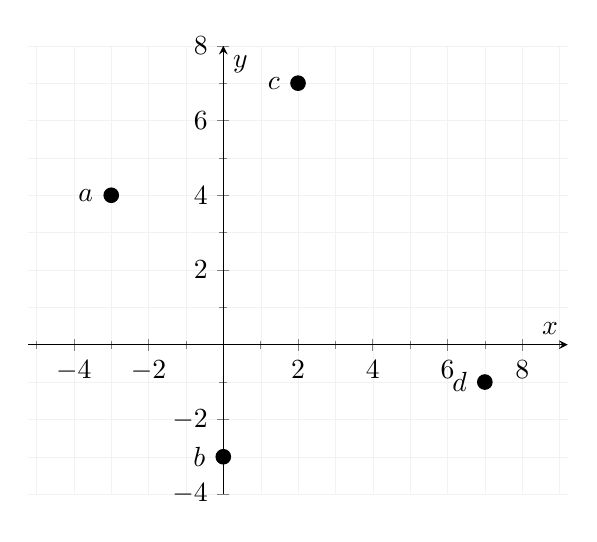
\begin{tikzpicture}
        \begin{axis}[my style,grid=both,
    grid style={line width=.1pt, draw=gray!10}, minor tick num=1, ymax=8, ymin=-4]

            \addplot[mark=*,only marks] coordinates {(-3,4)(0,-3)(2,7)(7,-1)};
            \node[label={180:{$a$}},circle,fill,inner sep=2pt] at (axis cs:-3,4) {};
            \node[label={180:{$b$}},circle,fill,inner sep=2pt] at (axis cs:0,-3) {};
            \node[label={180:{$c$}},circle,fill,inner sep=2pt] at (axis cs:2,7) {};
            \node[label={180:{$d$}},circle,fill,inner sep=2pt] at (axis cs:7,-1) {};
        \end{axis}
    \end{tikzpicture}

    What are the coordinates of point $a$? ($\answer{-3}$,$\answer{4}$)

    What are the coordinates of point $b$? ($\answer{0}$,$\answer{-3}$)

    What are the coordinates of point $c$? ($\answer{2}$,$\answer{7}$)

    What are the coordinates of point $d$? ($\answer{7}$,$\answer{-1}$)
\end{problem}

Match the graph manipulations to the appropriate \textbf{parent functions} (\textbf{NOTE: }not the actual function of the graph, but the parent function of the graph).

A) 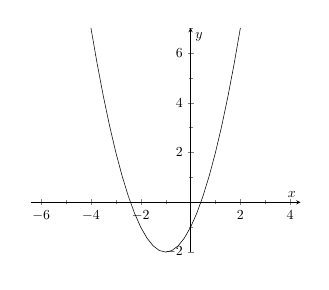
\begin{tikzpicture}[baseline={([yshift={-1ex}]current bounding box.north)}, scale=0.50]
    \begin{axis}[my style, minor tick num=1]
        \addplot[domain=-4:2]{3(x+1)^2-2};
    \end{axis}
\end{tikzpicture}
B) \begin{tikzpicture}[baseline={([yshift={-1ex}]current bounding box.north)}, scale=0.50]
    \begin{axis}[my style, minor tick num=1]
        \addplot[domain=-12:3]{2^(x+1) - 1};
    \end{axis}
\end{tikzpicture}

C) \begin{tikzpicture}[baseline={([yshift={-1ex}]current bounding box.north)}, scale=0.50]
    \begin{axis}[my style, minor tick num=1, xmin=0]
        \addplot[domain=1:5]{sqrt(x-1)};
    \end{axis}
\end{tikzpicture}
D) \begin{tikzpicture}[baseline={([yshift={-1ex}]current bounding box.north)}, scale=0.50]
    \begin{axis}[my style, minor tick num=1]
        \addplot[domain=-5:3]{4/5*x +2};
    \end{axis}
\end{tikzpicture}

E) \begin{tikzpicture}[baseline={([yshift={-1ex}]current bounding box.north)}, scale=0.50]
    \begin{axis}[my style, minor tick num=1]
        \addplot[domain=-3:3]{ln(x)};
    \end{axis}
\end{tikzpicture}
F) 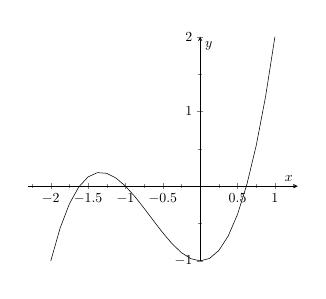
\begin{tikzpicture}[baseline={([yshift={-1ex}]current bounding box.north)}, scale=0.50]
    \begin{axis}[my style, minor tick num=1]
        \addplot[domain=-2:1]{x^3+2*x^2-1};
    \end{axis}
\end{tikzpicture}

\begin{problem}
    Which graph would most properly be said to have a parent function of $f(x) = x^2$

    Plot: $\answer{A}$
\end{problem}
\begin{problem}
    Which graph would most properly be said to have a parent function of $f(x) = \sqrt{x}$

     Plot: $\answer{C}$
\end{problem}
\begin{problem}
    Which graph would most properly be said to have a parent function of $f(x) = x$

    Plot: $\answer{D}$
\end{problem}
\begin{problem}
   Which graph would most properly be said to have a parent function of $f(x) = e^x$

    Plot: $\answer{B}$
\end{problem}
\begin{problem}
    Which graph would most properly be said to have a parent function of $f(x) = x^3$

    Plot: $\answer{F}$
\end{problem}
\begin{problem}
    Which graph would most properly be said to have a parent function of $f(x) = \ln(x)$

    Plot: $\answer{E}$
\end{problem}

\begin{problem}
    Which of the following are examples of independent variables?
    \begin{selectAll}
        \choice[correct]{$y$ = height of a wall. You are trying to calculate the surface area of a wall for painting.}
        \choice{$C$ = total cost of installing new windows. You are modeling the costs for building a house and you know each new window costs \$140.}
        \choice[correct]{$n$ = the number of katanas purchased by a martial arts school. You know each katana costs \$50 and you are trying to calculate the total cost to equip the school with katanas.}
        \choice{$P$ = the average price of gasoline from January 1, 2018 to August 1, 2018. You are running analysis on cost to consumers for driving in the first three quarters of 2018, \\
        given driving distance habits and gasoline price per gallon for each week.}
    \end{selectAll}
\end{problem}



\end{document}